\PassOptionsToPackage{unicode=true}{hyperref} % options for packages loaded elsewhere
\PassOptionsToPackage{hyphens}{url}
%
\documentclass[ignorenonframetext,]{beamer}
\usepackage{pgfpages}
\setbeamertemplate{caption}[numbered]
\setbeamertemplate{caption label separator}{: }
\setbeamercolor{caption name}{fg=normal text.fg}
\beamertemplatenavigationsymbolsempty
% Prevent slide breaks in the middle of a paragraph:
\widowpenalties 1 10000
\raggedbottom
\setbeamertemplate{part page}{
\centering
\begin{beamercolorbox}[sep=16pt,center]{part title}
  \usebeamerfont{part title}\insertpart\par
\end{beamercolorbox}
}
\setbeamertemplate{section page}{
\centering
\begin{beamercolorbox}[sep=12pt,center]{part title}
  \usebeamerfont{section title}\insertsection\par
\end{beamercolorbox}
}
\setbeamertemplate{subsection page}{
\centering
\begin{beamercolorbox}[sep=8pt,center]{part title}
  \usebeamerfont{subsection title}\insertsubsection\par
\end{beamercolorbox}
}
\AtBeginPart{
  \frame{\partpage}
}
\AtBeginSection{
  \ifbibliography
  \else
    \frame{\sectionpage}
  \fi
}
\AtBeginSubsection{
  \frame{\subsectionpage}
}
\usepackage{lmodern}
\usepackage{amssymb,amsmath}
\usepackage{ifxetex,ifluatex}
\usepackage{fixltx2e} % provides \textsubscript
\ifnum 0\ifxetex 1\fi\ifluatex 1\fi=0 % if pdftex
  \usepackage[T1]{fontenc}
  \usepackage[utf8]{inputenc}
  \usepackage{textcomp} % provides euro and other symbols
\else % if luatex or xelatex
  \usepackage{unicode-math}
  \defaultfontfeatures{Ligatures=TeX,Scale=MatchLowercase}
\fi
% use upquote if available, for straight quotes in verbatim environments
\IfFileExists{upquote.sty}{\usepackage{upquote}}{}
% use microtype if available
\IfFileExists{microtype.sty}{%
\usepackage[]{microtype}
\UseMicrotypeSet[protrusion]{basicmath} % disable protrusion for tt fonts
}{}
\IfFileExists{parskip.sty}{%
\usepackage{parskip}
}{% else
\setlength{\parindent}{0pt}
\setlength{\parskip}{6pt plus 2pt minus 1pt}
}
\usepackage{hyperref}
\hypersetup{
            pdftitle={Probability Distributions},
            pdfauthor={Robert W. Walker},
            pdfborder={0 0 0},
            breaklinks=true}
\urlstyle{same}  % don't use monospace font for urls
\newif\ifbibliography
\usepackage{color}
\usepackage{fancyvrb}
\newcommand{\VerbBar}{|}
\newcommand{\VERB}{\Verb[commandchars=\\\{\}]}
\DefineVerbatimEnvironment{Highlighting}{Verbatim}{commandchars=\\\{\}}
% Add ',fontsize=\small' for more characters per line
\usepackage{framed}
\definecolor{shadecolor}{RGB}{248,248,248}
\newenvironment{Shaded}{\begin{snugshade}}{\end{snugshade}}
\newcommand{\AlertTok}[1]{\textcolor[rgb]{0.94,0.16,0.16}{#1}}
\newcommand{\AnnotationTok}[1]{\textcolor[rgb]{0.56,0.35,0.01}{\textbf{\textit{#1}}}}
\newcommand{\AttributeTok}[1]{\textcolor[rgb]{0.77,0.63,0.00}{#1}}
\newcommand{\BaseNTok}[1]{\textcolor[rgb]{0.00,0.00,0.81}{#1}}
\newcommand{\BuiltInTok}[1]{#1}
\newcommand{\CharTok}[1]{\textcolor[rgb]{0.31,0.60,0.02}{#1}}
\newcommand{\CommentTok}[1]{\textcolor[rgb]{0.56,0.35,0.01}{\textit{#1}}}
\newcommand{\CommentVarTok}[1]{\textcolor[rgb]{0.56,0.35,0.01}{\textbf{\textit{#1}}}}
\newcommand{\ConstantTok}[1]{\textcolor[rgb]{0.00,0.00,0.00}{#1}}
\newcommand{\ControlFlowTok}[1]{\textcolor[rgb]{0.13,0.29,0.53}{\textbf{#1}}}
\newcommand{\DataTypeTok}[1]{\textcolor[rgb]{0.13,0.29,0.53}{#1}}
\newcommand{\DecValTok}[1]{\textcolor[rgb]{0.00,0.00,0.81}{#1}}
\newcommand{\DocumentationTok}[1]{\textcolor[rgb]{0.56,0.35,0.01}{\textbf{\textit{#1}}}}
\newcommand{\ErrorTok}[1]{\textcolor[rgb]{0.64,0.00,0.00}{\textbf{#1}}}
\newcommand{\ExtensionTok}[1]{#1}
\newcommand{\FloatTok}[1]{\textcolor[rgb]{0.00,0.00,0.81}{#1}}
\newcommand{\FunctionTok}[1]{\textcolor[rgb]{0.00,0.00,0.00}{#1}}
\newcommand{\ImportTok}[1]{#1}
\newcommand{\InformationTok}[1]{\textcolor[rgb]{0.56,0.35,0.01}{\textbf{\textit{#1}}}}
\newcommand{\KeywordTok}[1]{\textcolor[rgb]{0.13,0.29,0.53}{\textbf{#1}}}
\newcommand{\NormalTok}[1]{#1}
\newcommand{\OperatorTok}[1]{\textcolor[rgb]{0.81,0.36,0.00}{\textbf{#1}}}
\newcommand{\OtherTok}[1]{\textcolor[rgb]{0.56,0.35,0.01}{#1}}
\newcommand{\PreprocessorTok}[1]{\textcolor[rgb]{0.56,0.35,0.01}{\textit{#1}}}
\newcommand{\RegionMarkerTok}[1]{#1}
\newcommand{\SpecialCharTok}[1]{\textcolor[rgb]{0.00,0.00,0.00}{#1}}
\newcommand{\SpecialStringTok}[1]{\textcolor[rgb]{0.31,0.60,0.02}{#1}}
\newcommand{\StringTok}[1]{\textcolor[rgb]{0.31,0.60,0.02}{#1}}
\newcommand{\VariableTok}[1]{\textcolor[rgb]{0.00,0.00,0.00}{#1}}
\newcommand{\VerbatimStringTok}[1]{\textcolor[rgb]{0.31,0.60,0.02}{#1}}
\newcommand{\WarningTok}[1]{\textcolor[rgb]{0.56,0.35,0.01}{\textbf{\textit{#1}}}}
\usepackage{graphicx,grffile}
\makeatletter
\def\maxwidth{\ifdim\Gin@nat@width>\linewidth\linewidth\else\Gin@nat@width\fi}
\def\maxheight{\ifdim\Gin@nat@height>\textheight\textheight\else\Gin@nat@height\fi}
\makeatother
% Scale images if necessary, so that they will not overflow the page
% margins by default, and it is still possible to overwrite the defaults
% using explicit options in \includegraphics[width, height, ...]{}
\setkeys{Gin}{width=\maxwidth,height=\maxheight,keepaspectratio}
\setlength{\emergencystretch}{3em}  % prevent overfull lines
\providecommand{\tightlist}{%
  \setlength{\itemsep}{0pt}\setlength{\parskip}{0pt}}
\setcounter{secnumdepth}{0}

% set default figure placement to htbp
\makeatletter
\def\fps@figure{htbp}
\makeatother


\title{Probability Distributions}
\author{Robert W. Walker}
\date{2020-02-12}

\begin{document}
\frame{\titlepage}

\hypertarget{probability-the-logic-of-science}{%
\subsection{Probability: The Logic of
Science}\label{probability-the-logic-of-science}}

Jaynes presents a few core ideas and requirements for his rational
system. Probability emerges as the representation of circumstances in
which any given realization of a process is either TRUE or FALSE but
both are possible and expressable by probabilities

\begin{itemize}[<+->]
\tightlist
\item
  that sum to one for all events
\item
  are greater than or equal to zero for any given event
\end{itemize}

\begin{frame}

\end{frame}

\hypertarget{general-representation-of-probability}{%
\subsection{General Representation of
Probability}\label{general-representation-of-probability}}

Is of necessity two-dimensional,

\begin{itemize}[<+->]
\tightlist
\item
  We have \(x\) and
\item
  we have \(Pr(X=x)\) in one of two forms (Pr or f).
\end{itemize}

\begin{frame}

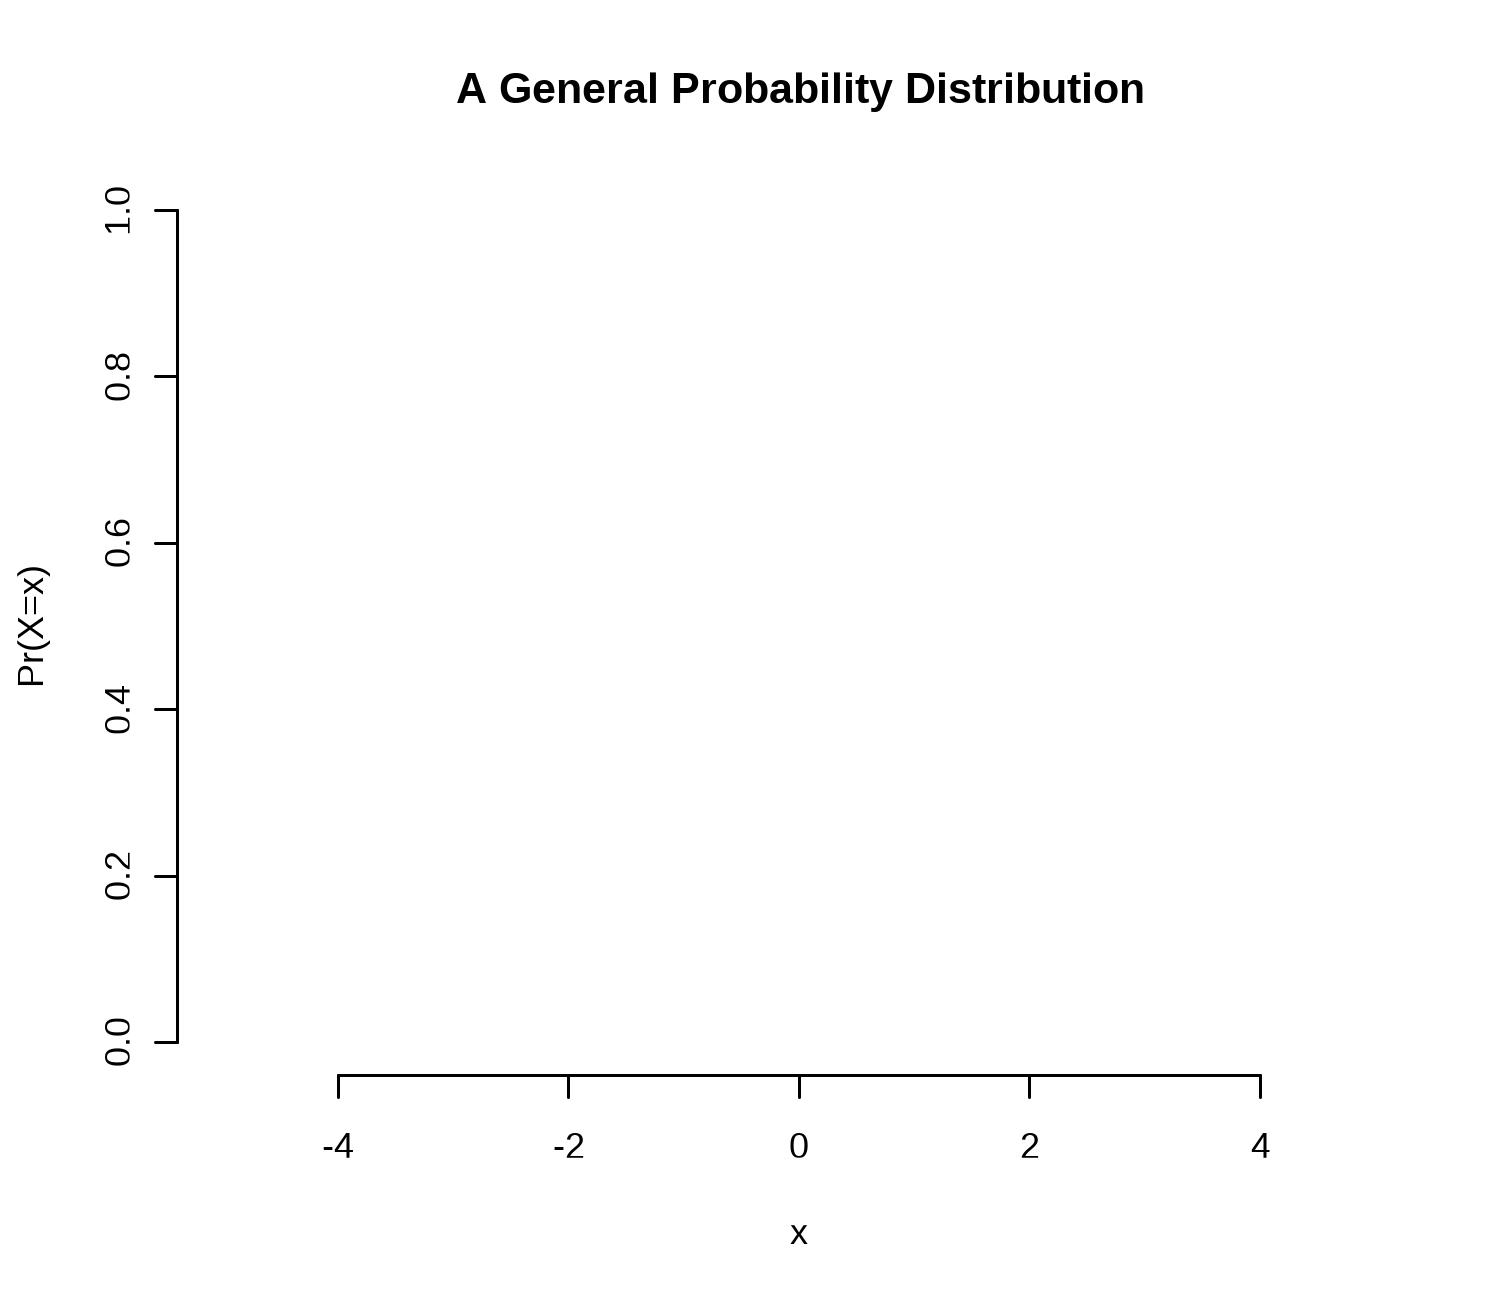
\includegraphics{Distributions_files/figure-beamer/P1-1.pdf}

\end{frame}

\begin{frame}

\end{frame}

\hypertarget{probability-distributions-of-two-forms}{%
\subsection{Probability Distributions of Two
Forms}\label{probability-distributions-of-two-forms}}

Our core concept is a probability distribution just as above. These come
in two forms for two types {[}discrete (qualitative){]} and continuous
(quantitative){]}:

\begin{itemize}[<+->]
\tightlist
\item
  Assumed
\item
  Derived
\end{itemize}

\begin{frame}

\end{frame}

\hypertarget{the-poster-and-examples}{%
\subsection{\texorpdfstring{\href{https://github.com/robertwwalker/DADMStuff/raw/master/Distribution-Poster.pdf}{The
Poster} and
Examples}{The Poster and Examples}}\label{the-poster-and-examples}}

Distributions are nouns. Sentences are incomplete without verbs --
parameters. We need both; it is for this reason that the former slide is
true. We do not always have a grounding for either the name or the
parameter.

\begin{frame}

\end{frame}

\hypertarget{continuous-vs.discrete-distributions}{%
\subsection{Continuous vs.~Discrete
Distributions}\label{continuous-vs.discrete-distributions}}

The differences are sums versus integrals. Why?

\begin{itemize}[<+->]
\tightlist
\item
  Histograms or\\
\item
  Density Plots
\end{itemize}

The probability of exactly any given value is zero on a true continuum.

\begin{frame}

Expectation

\[E(X) = \sum_{x \in X} x \cdot Pr(X=x)\]
\[E(X) = \int_{x \in X} x \cdot f(x)dx\]

Variance

\[E[(X-\mu)^2] = \sum_{x \in X} (x-\mu)^2 \cdot Pr(X=x)\]
\[E((X-\mu)^2) = \int_{x \in X} (x-\mu)^2 \cdot f(x)dx\]

\end{frame}

\hypertarget{the-z-transform}{%
\section{The z-transform}\label{the-z-transform}}

The generic z-transformation applied to a variable \(x\) centers
{[}mean\(\approx\) 0{]} and scales {[}std. dev. \(\approx\) variance
\(\approx\) 1{]} to \(z_{x}\) for population parameters. \(\approx\) is
approximately equal to.

\[ z = \frac{x - \mu}{\sigma} \]

\begin{frame}

In samples, the 0 and 1 are exact; these are features of the mean and
\emph{degrees of freedom} from last time.

\[ z = \frac{x - \overline{x}}{s_{x}} \].

where \(\overline{x}\) is the sample mean of \(x\) and \(s_{x}\) is the
sample standard deviation of \(x\). Take the example of earnings.

\end{frame}

\begin{frame}

Suppose earnings in a community have mean 55,000 and standard deviation
10,000. This is in dollars. Suppose I earn 75,000 dollars. First, if we
take the top part of the fraction in the \(z\) equation, we see that I
earn 20,000 dollars more than the average (75000 - 55000). Finishing the
calculation of z, I would divide that 20,000 dollars by 10,000 dollars
per standard deviation. Let's show that.

\[ z = \frac{75000 dollars - 55000 dollars}{\frac{10000 dollars}{SD}} = +2 SD \].

I am 2 standard deviations above the average (the +) earnings. All \(z\)
does is re-scale the original data to standard deviations with zero as
the mean.

\end{frame}

\begin{frame}

Suppose I earn 35,000. That makes me 20,000 below the average and gives
me a z score of -2. I am 2 standard deviations below average (the -)
earnings.

\(z\) is an easy way to assess symmetry. The mean of z is always zero
but the distribution of z to the left and right of zero is informative.
If they are roughly even, then symmetry is likely. If the signs are
uneven, then symmetry is unlikely. In R, \(z\) is automated with the
\emph{scale()} command. The last line uses a table and the \emph{sign}
command to show me the positive and negative z.

\end{frame}

\begin{frame}[fragile]

\begin{Shaded}
\begin{Highlighting}[]
\CommentTok{# Generate random normal income}
\NormalTok{Hypo.Income <-}\StringTok{ }\KeywordTok{rnorm}\NormalTok{(}\DecValTok{1000}\NormalTok{, }\DecValTok{55000}\NormalTok{, }\DecValTok{10000}\NormalTok{)}
\CommentTok{# z-transform income [mean 55000ish, std. dev. 10000ish]}
\NormalTok{z.Income <-}\StringTok{ }\KeywordTok{scale}\NormalTok{(Hypo.Income)}
\CommentTok{# Combine them into a data.frame}
\NormalTok{Income <-}\StringTok{ }\KeywordTok{data.frame}\NormalTok{(Hypo.Income,z.Income)}
\CommentTok{# Show the data.frame}
\KeywordTok{head}\NormalTok{(Income)}
\end{Highlighting}
\end{Shaded}

\begin{verbatim}
##   Hypo.Income   z.Income
## 1    71700.80  1.6890125
## 2    60749.91  0.5791407
## 3    58941.91  0.3959002
## 4    34258.31 -2.1057800
## 5    48504.53 -0.6619266
## 6    49148.68 -0.5966424
\end{verbatim}

\begin{Shaded}
\begin{Highlighting}[]
\KeywordTok{table}\NormalTok{(}\KeywordTok{sign}\NormalTok{(z.Income))}
\end{Highlighting}
\end{Shaded}

\begin{verbatim}
## 
##  -1   1 
## 515 485
\end{verbatim}

\end{frame}

\hypertarget{probability-distributions}{%
\section{Probability Distributions}\label{probability-distributions}}

Distributions in R are defined by four core parts:

\begin{itemize}[<+->]
\tightlist
\item
  r, for random variables
\item
  p, for cumulative probability (given x) {[}counting from left{]}
  \(Pr(X\leq x)\)
\item
  d, for density/probability that \(Pr(X=x)\) or \(f(x)\)
\item
  q, for quantile (given p): x such that \(Pr(X\leq q)=p\)
\end{itemize}

\hypertarget{a-grape-escape}{%
\subsection{A Grape Escape?}\label{a-grape-escape}}

A filling process is supposed to fill jars with 16 ounces of grape
jelly, according to the label, and regulations require that each jar
contain between 15.95 and 16.05 ounces.

\begin{enumerate}[<+->]
\tightlist
\item
  \emph{Suppose that the uniform random process of filling in known to
  fill between 15.9 and 16.1 ounces uniformly.}
\end{enumerate}

\begin{itemize}[<+->]
\tightlist
\item
  Plot the histogram of 1000 simulated values. NB: \emph{unif} is the
  noun with boundaries a (default 0) and b(default 1).
\end{itemize}

\begin{Shaded}
\begin{Highlighting}[]
\NormalTok{Jars <-}\StringTok{ }\KeywordTok{runif}\NormalTok{(}\DecValTok{1000}\NormalTok{, }\FloatTok{15.9}\NormalTok{, }\FloatTok{16.1}\NormalTok{)}
\KeywordTok{hist}\NormalTok{(Jars)}
\end{Highlighting}
\end{Shaded}

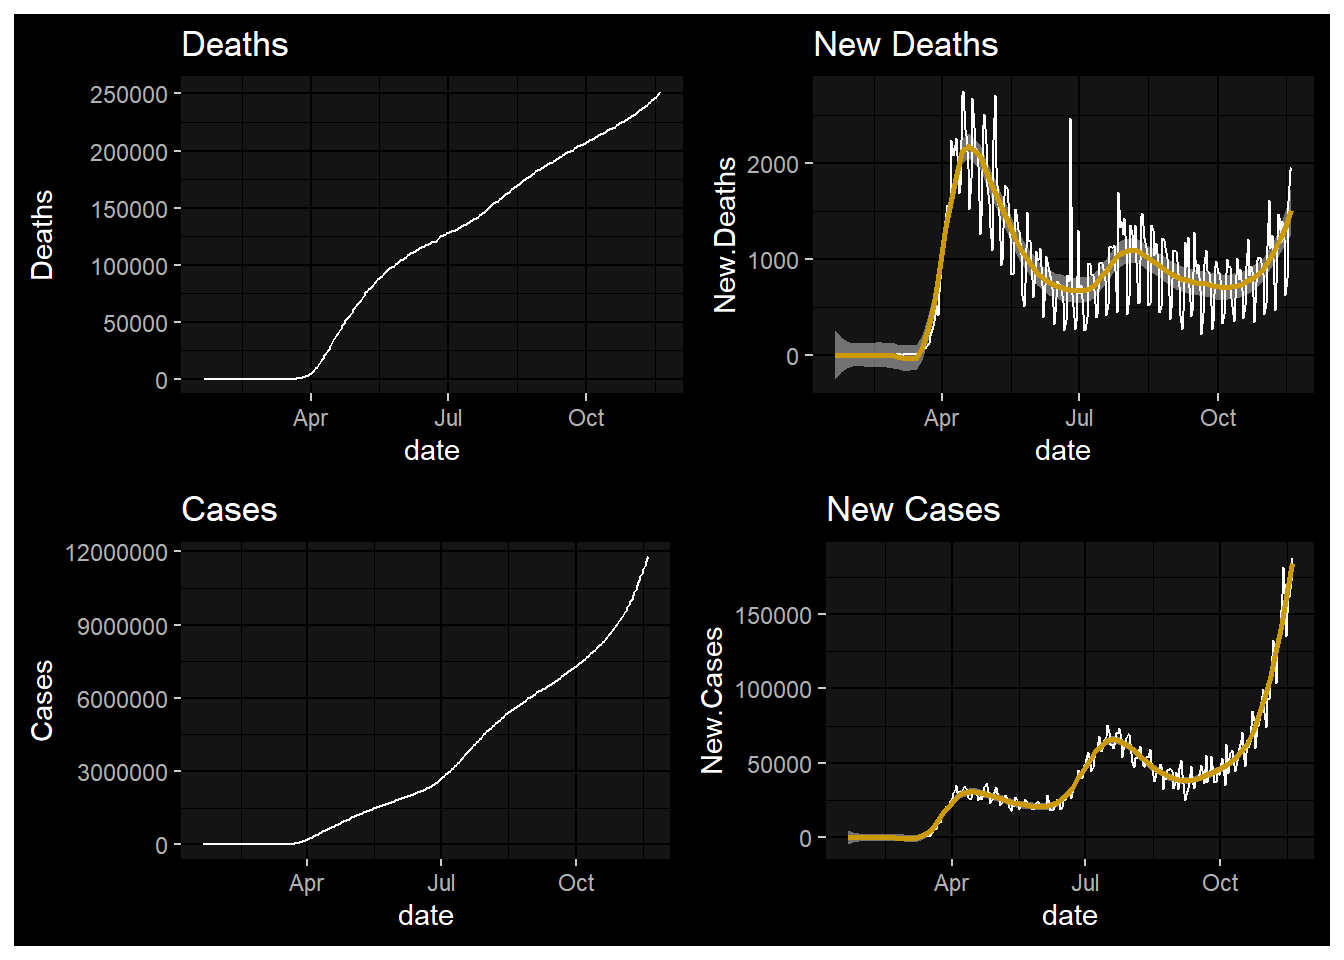
\includegraphics{Distributions_files/figure-beamer/unnamed-chunk-1-1.pdf}

\begin{itemize}[<+->]
\tightlist
\item
  What is the probability that a random jar is outside of requirements?
\end{itemize}

\textbf{Exactly? 50 percent because 25 percent are between 15.9 and
15.95 and 25 percent are between 16.05 and 16.1.}

\begin{Shaded}
\begin{Highlighting}[]
\KeywordTok{table}\NormalTok{(Jars }\OperatorTok{<}\StringTok{ }\FloatTok{15.95} \OperatorTok{|}\StringTok{ }\NormalTok{Jars }\OperatorTok{>}\StringTok{ }\FloatTok{16.05}\NormalTok{) }\CommentTok{# | captures or}
\end{Highlighting}
\end{Shaded}

\begin{verbatim}
## 
## FALSE  TRUE 
##   526   474
\end{verbatim}

\begin{itemize}[<+->]
\tightlist
\item
  Scale (z) the jars and summarise them.
\end{itemize}

\begin{Shaded}
\begin{Highlighting}[]
\KeywordTok{summary}\NormalTok{(}\KeywordTok{scale}\NormalTok{(Jars))}
\end{Highlighting}
\end{Shaded}

\begin{verbatim}
##        V1          
##  Min.   :-1.80038  
##  1st Qu.:-0.83138  
##  Median :-0.01907  
##  Mean   : 0.00000  
##  3rd Qu.: 0.86235  
##  Max.   : 1.75310
\end{verbatim}

\begin{Shaded}
\begin{Highlighting}[]
\KeywordTok{sd}\NormalTok{(}\KeywordTok{scale}\NormalTok{(Jars))}
\end{Highlighting}
\end{Shaded}

\begin{verbatim}
## [1] 1
\end{verbatim}

\begin{frame}[fragile]

\begin{enumerate}[<+->]
\setcounter{enumi}{1}
\tightlist
\item
  \emph{The mean of the normal random process of filling is known to be
  16.004 ounces with standard deviation 0.028 ounces.}
\end{enumerate}

\begin{itemize}[<+->]
\tightlist
\item
  What is the probability that a random jar is outside of requirements?
  NB: \emph{norm} is the noun with mean (default 0) and sd (default 1).
\end{itemize}

\begin{Shaded}
\begin{Highlighting}[]
\KeywordTok{pnorm}\NormalTok{(}\FloatTok{15.95}\NormalTok{, }\FloatTok{16.004}\NormalTok{, }\FloatTok{0.028}\NormalTok{) }\OperatorTok{+}\StringTok{ }\KeywordTok{pnorm}\NormalTok{(}\FloatTok{16.05}\NormalTok{, }\FloatTok{16.004}\NormalTok{, }\FloatTok{0.028}\NormalTok{, }\DataTypeTok{lower.tail=}\OtherTok{FALSE}\NormalTok{)}
\end{Highlighting}
\end{Shaded}

\begin{verbatim}
## [1] 0.07709829
\end{verbatim}

\begin{itemize}[<+->]
\tightlist
\item
  What is the probability that a random jar contains more than 16.1
  ounces?
\end{itemize}

\begin{Shaded}
\begin{Highlighting}[]
\DecValTok{1}\OperatorTok{-}\KeywordTok{pnorm}\NormalTok{(}\FloatTok{16.1}\NormalTok{, }\FloatTok{16.004}\NormalTok{, }\FloatTok{0.028}\NormalTok{)}
\end{Highlighting}
\end{Shaded}

\begin{verbatim}
## [1] 0.0003033834
\end{verbatim}

\begin{itemize}[<+->]
\tightlist
\item
  What is the probability that a random jar contains less than 16.04
  ounces?
\end{itemize}

\begin{Shaded}
\begin{Highlighting}[]
\KeywordTok{pnorm}\NormalTok{(}\FloatTok{16.04}\NormalTok{, }\FloatTok{16.004}\NormalTok{, }\FloatTok{0.028}\NormalTok{)}
\end{Highlighting}
\end{Shaded}

\begin{verbatim}
## [1] 0.9007286
\end{verbatim}

\begin{itemize}[<+->]
\tightlist
\item
  95\% of jars, given a normal, will contain between XXX and XXX ounces
  of jelly.
\end{itemize}

\begin{Shaded}
\begin{Highlighting}[]
\KeywordTok{qnorm}\NormalTok{(}\KeywordTok{c}\NormalTok{(}\FloatTok{0.025}\NormalTok{,}\FloatTok{0.975}\NormalTok{), }\FloatTok{16.004}\NormalTok{, }\FloatTok{0.028}\NormalTok{)}
\end{Highlighting}
\end{Shaded}

\begin{verbatim}
## [1] 15.94912 16.05888
\end{verbatim}

\begin{itemize}[<+->]
\tightlist
\item
  The bottom 5\% of jars contain, at most, XXX ounces of jelly.
\end{itemize}

\begin{Shaded}
\begin{Highlighting}[]
\KeywordTok{qnorm}\NormalTok{(}\FloatTok{0.05}\NormalTok{, }\FloatTok{16.004}\NormalTok{, }\FloatTok{0.028}\NormalTok{)}
\end{Highlighting}
\end{Shaded}

\begin{verbatim}
## [1] 15.95794
\end{verbatim}

\begin{itemize}[<+->]
\tightlist
\item
  The top 25\% of jars contain at least XXX ounces of jelly.
\end{itemize}

\begin{Shaded}
\begin{Highlighting}[]
\KeywordTok{qnorm}\NormalTok{(}\FloatTok{0.75}\NormalTok{, }\FloatTok{16.004}\NormalTok{, }\FloatTok{0.028}\NormalTok{)}
\end{Highlighting}
\end{Shaded}

\begin{verbatim}
## [1] 16.02289
\end{verbatim}

\end{frame}

\hypertarget{scottish-pounds}{%
\subsection{Scottish Pounds}\label{scottish-pounds}}

\emph{Informal surveys suggest that 15\% of Essex shopkeepers will not
accept Scottish pounds. There are approximately 200 shops in the general
High Street square.}

\begin{enumerate}[<+->]
\tightlist
\item
  Draw a plot of the distribution and the cumulative distribution of
  shopkeepers that do not accept Scottish pounds.
\end{enumerate}

\begin{Shaded}
\begin{Highlighting}[]
\KeywordTok{plot}\NormalTok{(}\DataTypeTok{x=}\KeywordTok{seq}\NormalTok{(}\DecValTok{0}\NormalTok{,}\DecValTok{200}\NormalTok{), }\DataTypeTok{y=}\KeywordTok{pbinom}\NormalTok{(}\KeywordTok{seq}\NormalTok{(}\DecValTok{0}\NormalTok{,}\DecValTok{200}\NormalTok{), }\DataTypeTok{size=}\DecValTok{200}\NormalTok{, }\FloatTok{0.15}\NormalTok{), }\DataTypeTok{xlab=}\StringTok{"Refusers"}\NormalTok{, }\DataTypeTok{ylab=}\StringTok{"Prob. of x or Less Refusers"}\NormalTok{)}
\end{Highlighting}
\end{Shaded}

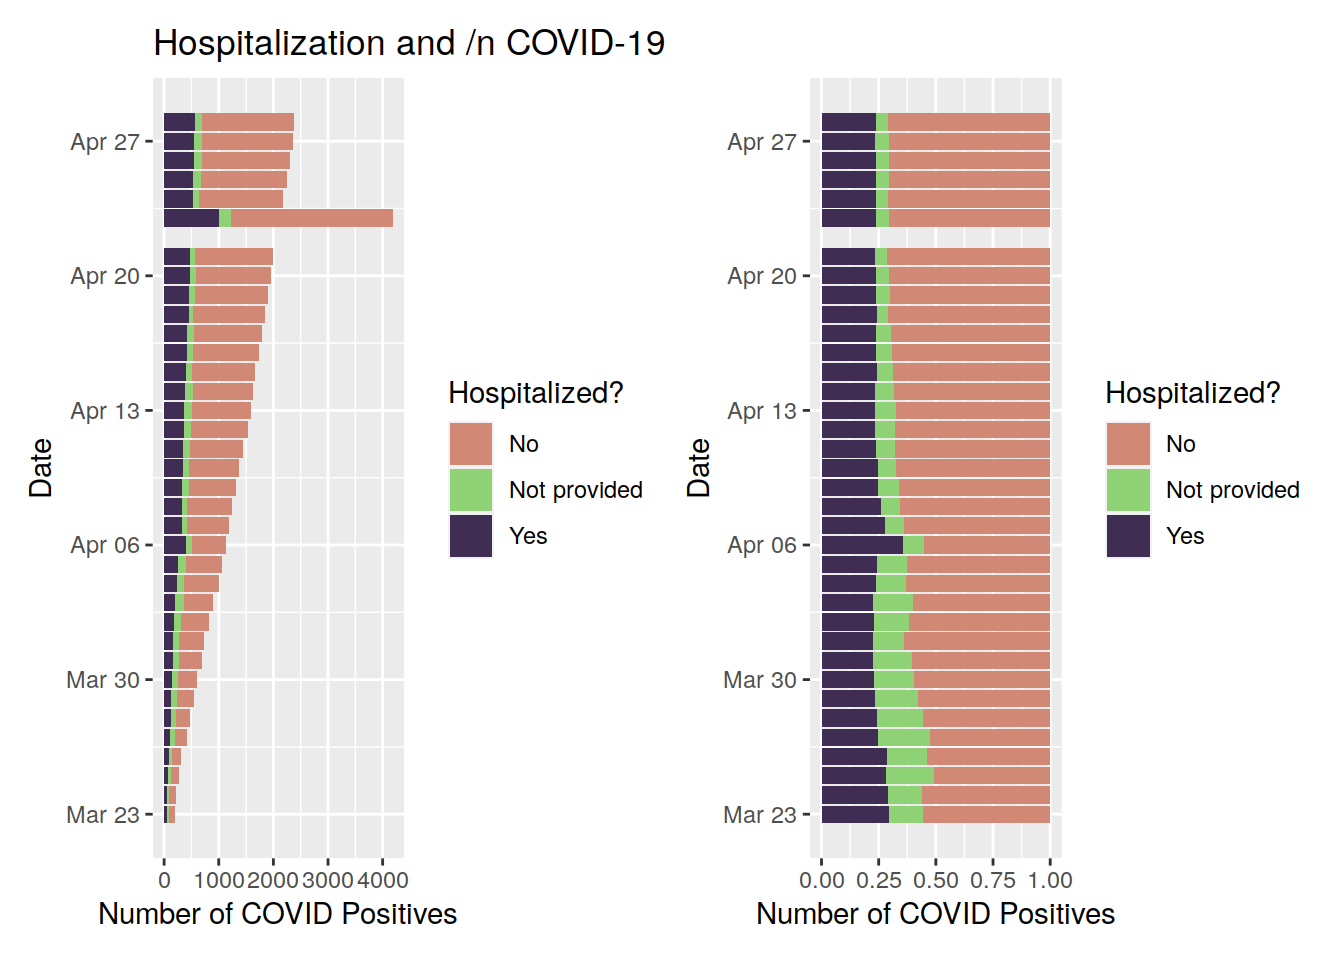
\includegraphics{Distributions_files/figure-beamer/unnamed-chunk-10-1.pdf}

\begin{enumerate}[<+->]
\setcounter{enumi}{1}
\tightlist
\item
  What is the probability that 24 or fewer will not accept Scottish
  pounds?
\end{enumerate}

\begin{Shaded}
\begin{Highlighting}[]
\KeywordTok{pbinom}\NormalTok{(}\DecValTok{24}\NormalTok{, }\DecValTok{200}\NormalTok{, }\FloatTok{0.15}\NormalTok{)}
\end{Highlighting}
\end{Shaded}

\begin{verbatim}
## [1] 0.1368173
\end{verbatim}

\begin{enumerate}[<+->]
\setcounter{enumi}{2}
\tightlist
\item
  What is the probability that 25 or more shopkeepers will not accept
  Scottish pounds?
\end{enumerate}

\begin{Shaded}
\begin{Highlighting}[]
\DecValTok{1}\OperatorTok{-}\KeywordTok{pbinom}\NormalTok{(}\DecValTok{24}\NormalTok{, }\DecValTok{200}\NormalTok{, }\FloatTok{0.15}\NormalTok{)}
\end{Highlighting}
\end{Shaded}

\begin{verbatim}
## [1] 0.8631827
\end{verbatim}

\begin{enumerate}[<+->]
\setcounter{enumi}{3}
\tightlist
\item
  With probability 0.9 {[}90 percent{]}, XXX or fewer shopkeepers will
  not accept Scottish pounds.
\end{enumerate}

\begin{Shaded}
\begin{Highlighting}[]
\KeywordTok{qbinom}\NormalTok{(}\FloatTok{0.9}\NormalTok{, }\DecValTok{200}\NormalTok{, }\FloatTok{0.15}\NormalTok{)}
\end{Highlighting}
\end{Shaded}

\begin{verbatim}
## [1] 37
\end{verbatim}

\begin{enumerate}[<+->]
\setcounter{enumi}{4}
\tightlist
\item
  {[}Geometric{]} Plot 1000 random draws of ``How many vendors until one
  refuses my Scottish pounds?''
\end{enumerate}

\begin{Shaded}
\begin{Highlighting}[]
\KeywordTok{hist}\NormalTok{(}\KeywordTok{rgeom}\NormalTok{(}\DecValTok{1000}\NormalTok{, }\FloatTok{0.15}\NormalTok{), }\DataTypeTok{breaks=}\DecValTok{30}\NormalTok{)}
\end{Highlighting}
\end{Shaded}

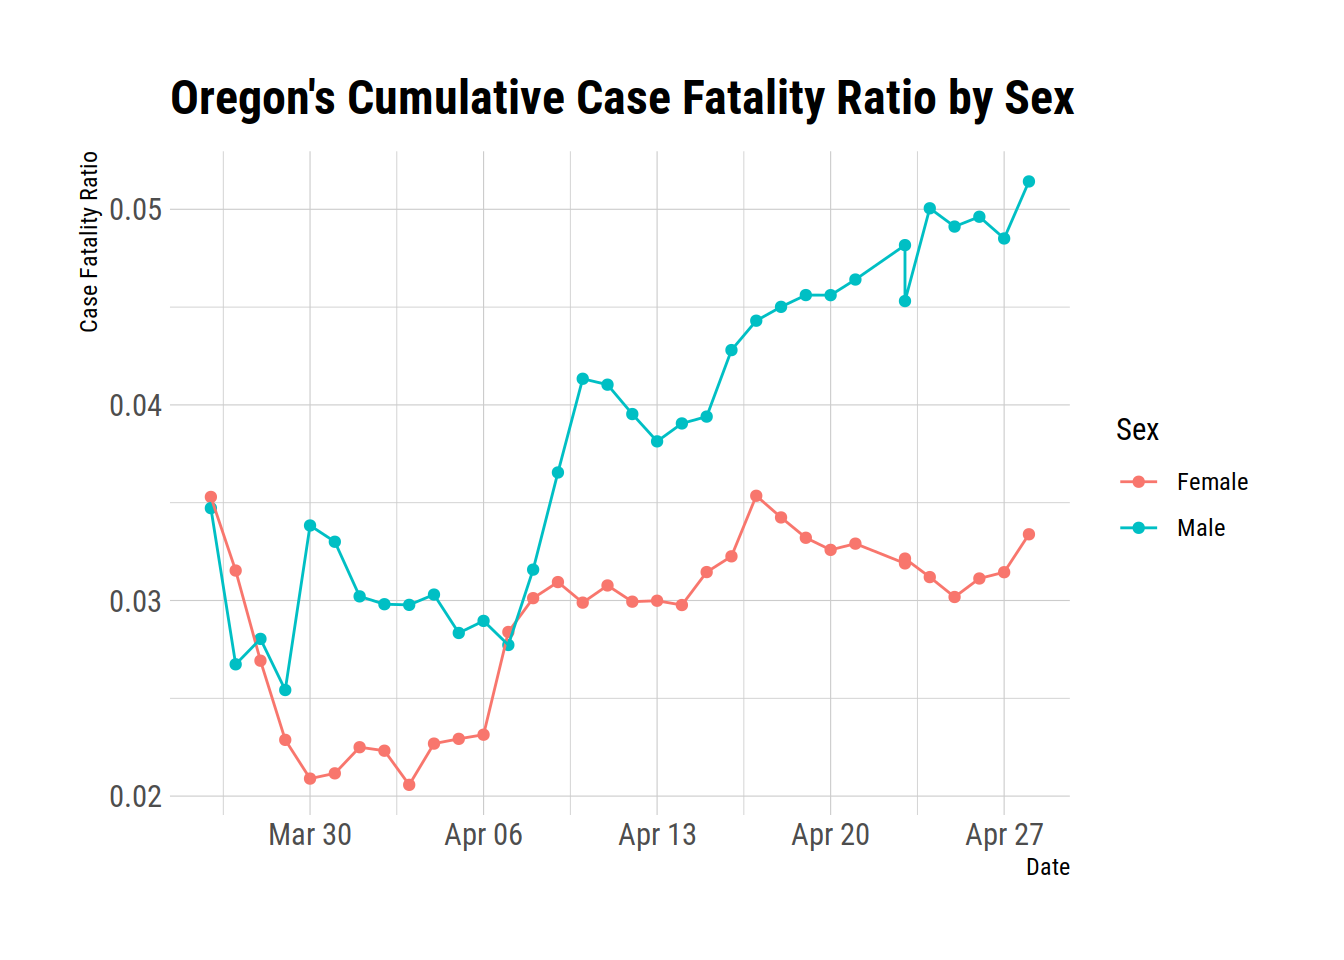
\includegraphics{Distributions_files/figure-beamer/unnamed-chunk-14-1.pdf}

We could also do something like.

\begin{Shaded}
\begin{Highlighting}[]
\KeywordTok{plot}\NormalTok{(}\KeywordTok{seq}\NormalTok{(}\DecValTok{0}\NormalTok{,}\DecValTok{60}\NormalTok{), }\KeywordTok{pgeom}\NormalTok{(}\KeywordTok{seq}\NormalTok{(}\DecValTok{0}\NormalTok{,}\DecValTok{60}\NormalTok{), }\FloatTok{0.15}\NormalTok{))}
\end{Highlighting}
\end{Shaded}

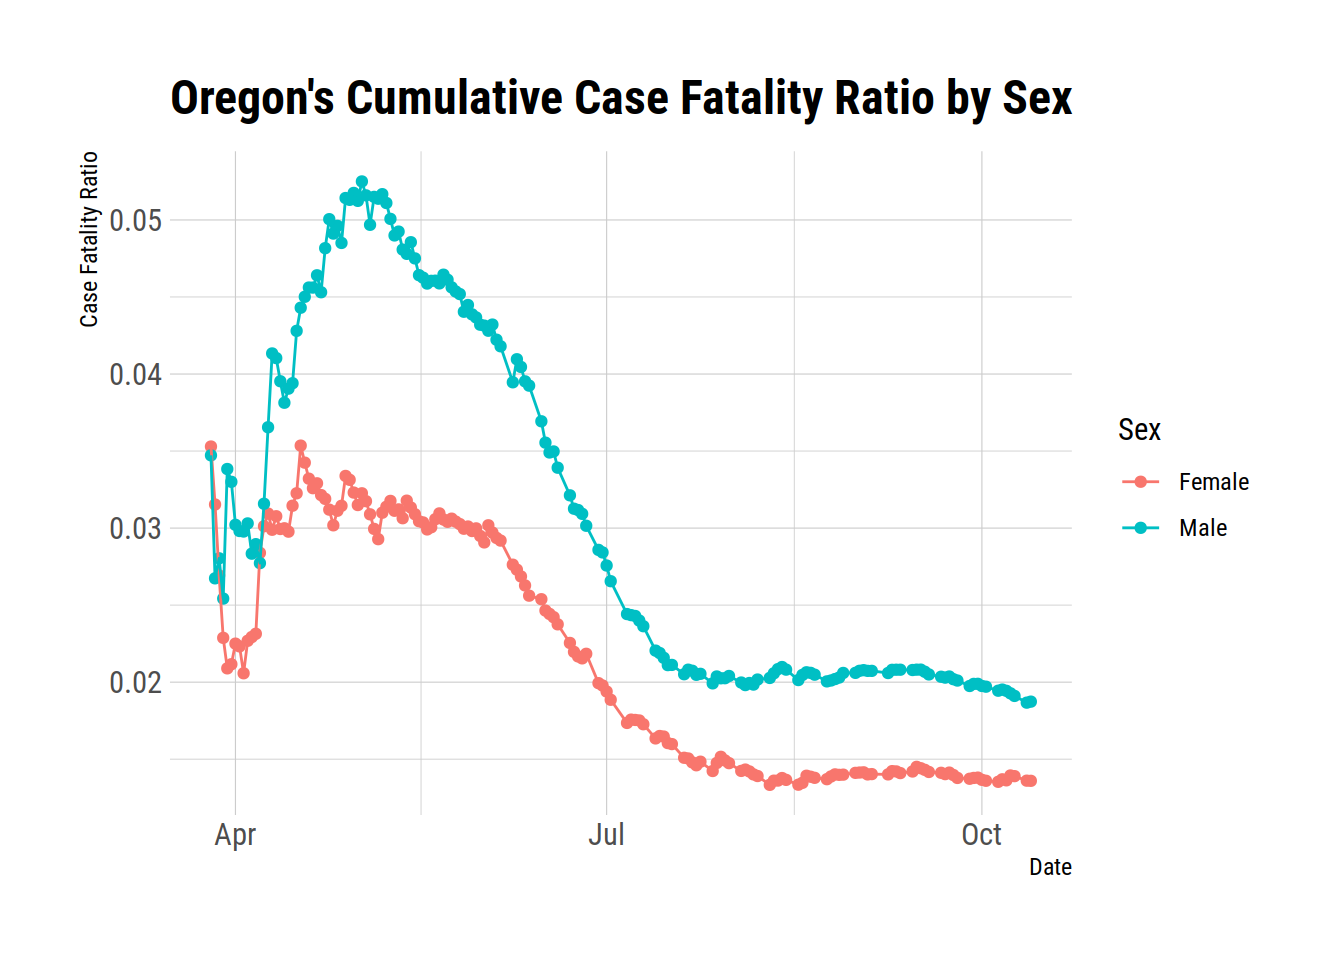
\includegraphics{Distributions_files/figure-beamer/unnamed-chunk-15-1.pdf}

\hypertarget{the-median-is-a-binomial-with-p0.5}{%
\subsection{The Median is a Binomial with
p=0.5}\label{the-median-is-a-binomial-with-p0.5}}

Interestingly, any given observation has a 50-50 chance of being
\emph{over} or \emph{under} the median. Suppose that I have five
datum.\\
1. What is the probability that all are under?

\begin{Shaded}
\begin{Highlighting}[]
\KeywordTok{pbinom}\NormalTok{(}\DecValTok{0}\NormalTok{,}\DataTypeTok{size=}\DecValTok{5}\NormalTok{, }\DataTypeTok{p=}\FloatTok{0.5}\NormalTok{)}
\end{Highlighting}
\end{Shaded}

\begin{verbatim}
## [1] 0.03125
\end{verbatim}

\begin{enumerate}[<+->]
\setcounter{enumi}{1}
\tightlist
\item
  What is the probability that all are over?
\end{enumerate}

\begin{Shaded}
\begin{Highlighting}[]
\KeywordTok{dbinom}\NormalTok{(}\DecValTok{5}\NormalTok{,}\DataTypeTok{size=}\DecValTok{5}\NormalTok{, }\DataTypeTok{p=}\FloatTok{0.5}\NormalTok{)}
\end{Highlighting}
\end{Shaded}

\begin{verbatim}
## [1] 0.03125
\end{verbatim}

\begin{enumerate}[<+->]
\setcounter{enumi}{2}
\tightlist
\item
  What is the probability that the median is somewhere in between our
  smallest and largest sampled values?
\end{enumerate}

\textbf{Everything else}.

This \emph{Rule of Five} often credited to Hubbard is handy.

\begin{frame}[fragile]{Air Traffic Controllers}
\protect\hypertarget{air-traffic-controllers}{}

FAA Decision: Expend or do not expend scarce resources investigating
claimed staffing shortages at the Cleveland Air Route Traffic Control
Center.

Essential facts: The Cleveland ARTCC is the US's busiest in routing
cross-country air traffic. In mid-August of 1998, it was reported that
the first week of August experienced 3 errors in a one week period; an
error occurs when flights come within five miles of one another by
horizontal distance or 2000 feet by vertical distance. The Controller's
union claims a staffing shortage though other factors could be
responsible. 21 errors per year (21/52 errors per week) has been the
norm in Cleveland for over a decade.

\begin{enumerate}[<+->]
\tightlist
\item
  Plot a histogram of 1000 random weeks. NB: \emph{pois} is the noun
  with no default for \(\lambda\) -- the arrival rate.
\end{enumerate}

\begin{Shaded}
\begin{Highlighting}[]
\KeywordTok{hist}\NormalTok{(}\KeywordTok{rpois}\NormalTok{(}\DecValTok{1000}\NormalTok{, }\DecValTok{21}\OperatorTok{/}\DecValTok{52}\NormalTok{))}
\end{Highlighting}
\end{Shaded}

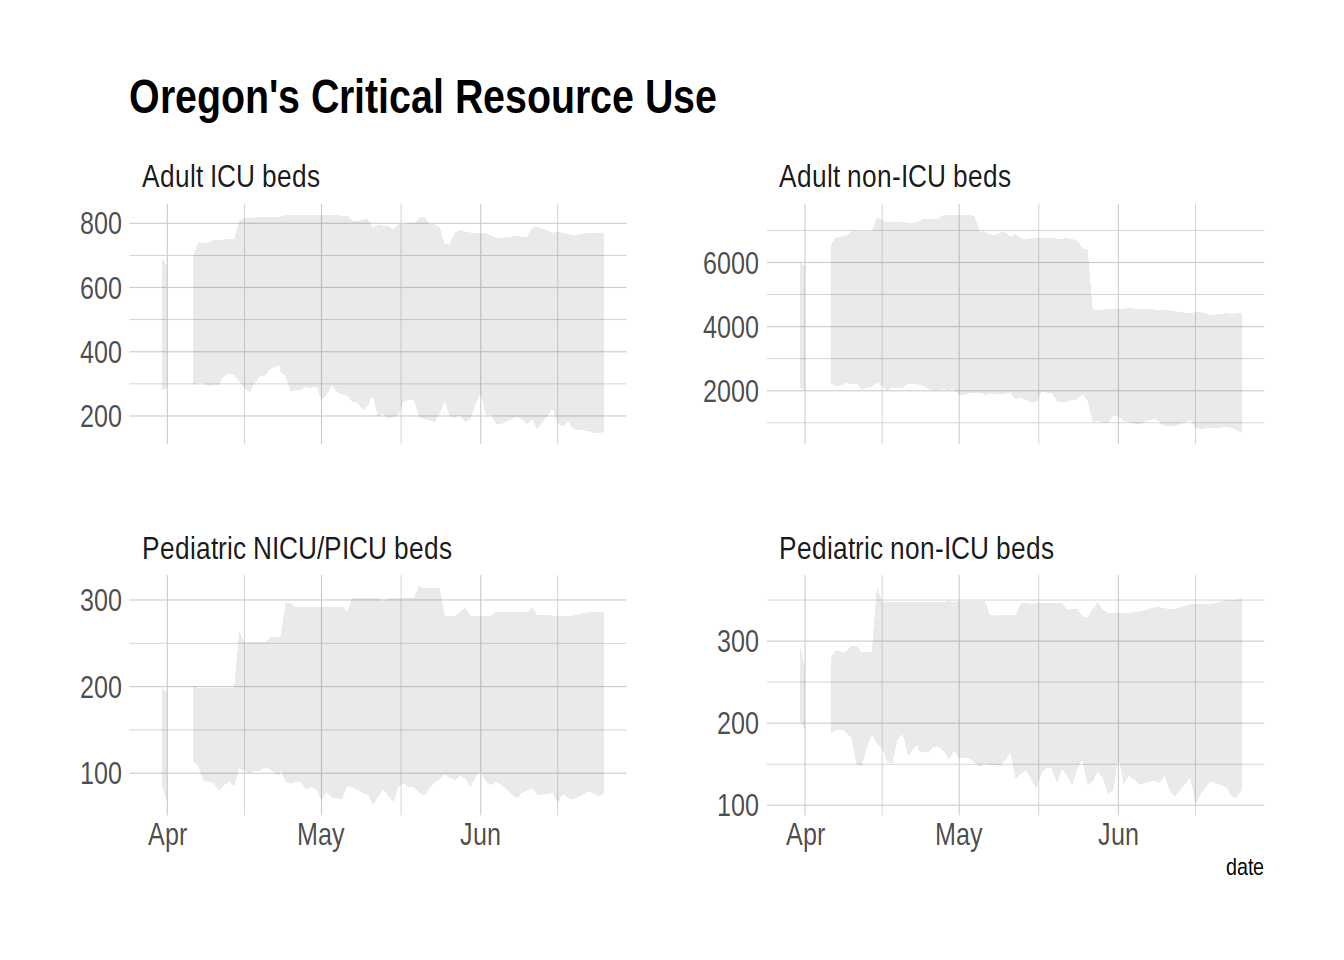
\includegraphics{Distributions_files/figure-beamer/unnamed-chunk-18-1.pdf}

\begin{itemize}[<+->]
\tightlist
\item
  Plot a sequence on the x axis from 0 to 5 and the probability of that
  or fewer incidents along the y. \emph{seq(0,5)}
\end{itemize}

\begin{Shaded}
\begin{Highlighting}[]
\KeywordTok{plot}\NormalTok{(}\KeywordTok{seq}\NormalTok{(}\DecValTok{0}\NormalTok{,}\DecValTok{5}\NormalTok{),}\KeywordTok{ppois}\NormalTok{(}\KeywordTok{seq}\NormalTok{(}\DecValTok{0}\NormalTok{,}\DecValTok{5}\NormalTok{), }\DecValTok{21}\OperatorTok{/}\DecValTok{52}\NormalTok{), }\DataTypeTok{ylim=}\KeywordTok{c}\NormalTok{(}\DecValTok{0}\NormalTok{,}\DecValTok{1}\NormalTok{))}
\end{Highlighting}
\end{Shaded}

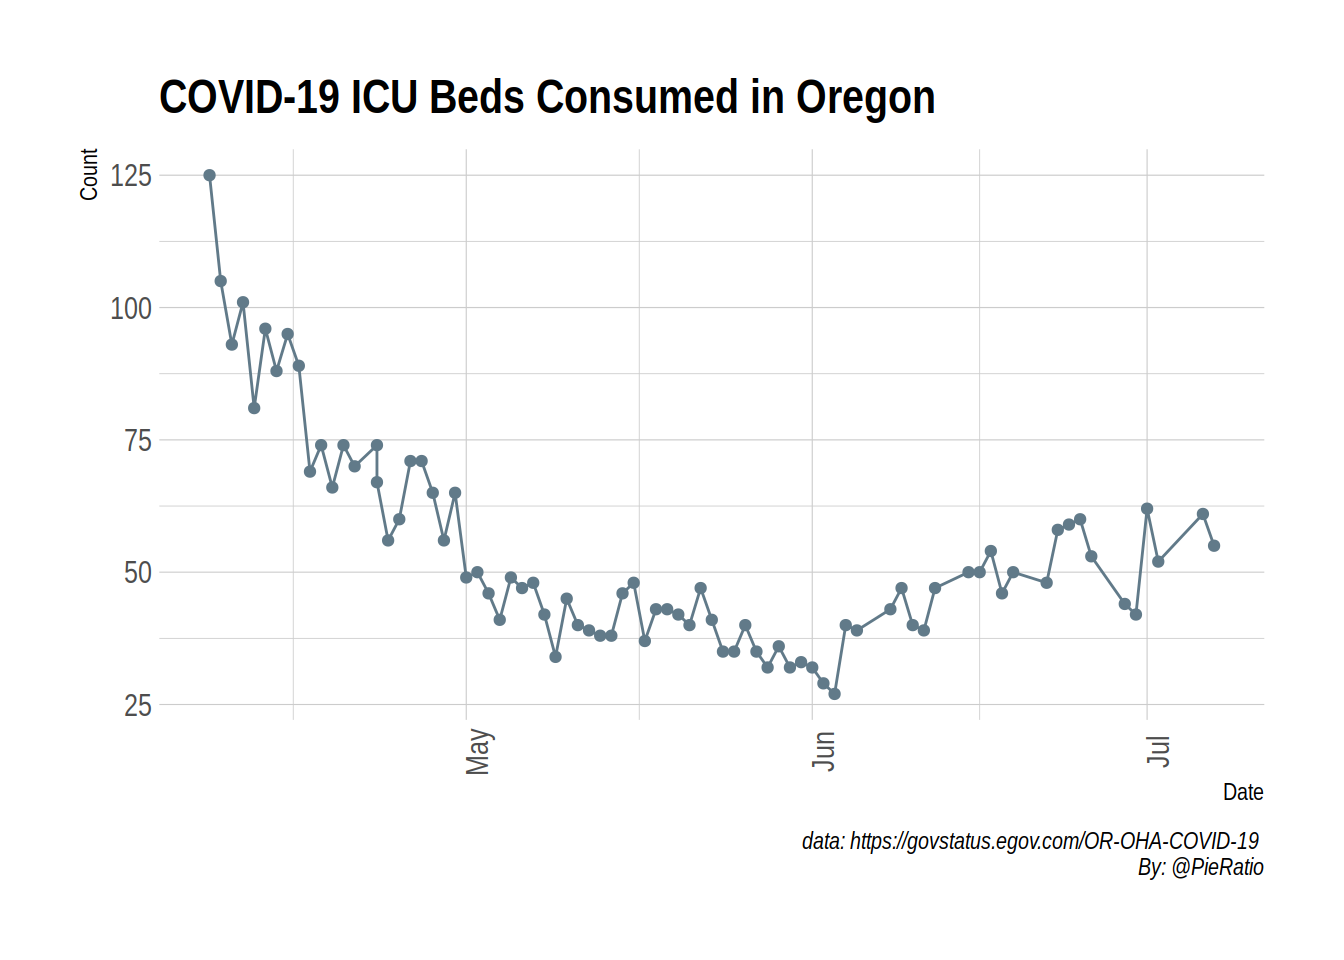
\includegraphics{Distributions_files/figure-beamer/unnamed-chunk-19-1.pdf}

\begin{enumerate}[<+->]
\setcounter{enumi}{1}
\item
  What would you do and why? \emph{Not impossible}
\item
  After analyzing the initial data, you discover that the first two
  weeks of August have experienced 6 errors. What would you now decide?
  \emph{Well, once is 0.0081342.} Twice, at random, is that squared. We
  have a problem.
\end{enumerate}

\end{frame}

\begin{frame}{Deaths by Horse Kick in the Prussian cavalry?}
\protect\hypertarget{deaths-by-horse-kick-in-the-prussian-cavalry}{}

\end{frame}

\begin{frame}[fragile]{{[}Given time{]} A Less Basic Monte Carlo
Simulation:}
\protect\hypertarget{given-time-a-less-basic-monte-carlo-simulation}{}

\begin{enumerate}[<+->]
\tightlist
\item
  Customers arriving at a car dealership at a rate of 6 per hour.
\item
  Each customer has a 15\% probability of making a purchase.
\item
  Purchasers yield {[}this part is harder{]}:
\end{enumerate}

\begin{itemize}[<+->]
\tightlist
\item
  Uniform profits over the interval \$1000-\$3000.
\item
  Normal profits that average \$1500 with standard deviation \$500.
\end{itemize}

\begin{Shaded}
\begin{Highlighting}[]
\NormalTok{Customers <-}\StringTok{ }\KeywordTok{rpois}\NormalTok{(}\DecValTok{1000}\NormalTok{, }\DecValTok{6}\NormalTok{) }\CommentTok{# Customers ~ Poisson(6)}
\NormalTok{Purchasers <-}\StringTok{ }\KeywordTok{rbinom}\NormalTok{(}\DecValTok{1000}\NormalTok{, }\DataTypeTok{size=}\NormalTok{Customers, }\DataTypeTok{prob=}\FloatTok{0.15}\NormalTok{) }\CommentTok{# P ~ Binomial(Customers,0.15)}
\CommentTok{# Next part needs a coding trick.  For each row [of 1000], I want sum the Profits given Purchasers random draws.}
\NormalTok{Profits.U <-}\StringTok{ }\KeywordTok{sapply}\NormalTok{(}\KeywordTok{c}\NormalTok{(}\DecValTok{1}\OperatorTok{:}\DecValTok{1000}\NormalTok{), }\ControlFlowTok{function}\NormalTok{(x) \{ }\KeywordTok{sum}\NormalTok{(}\KeywordTok{runif}\NormalTok{(Purchasers[[x]], }\DecValTok{1000}\NormalTok{, }\DecValTok{3000}\NormalTok{))\} )}
\NormalTok{Profits.N <-}\StringTok{ }\KeywordTok{sapply}\NormalTok{(}\KeywordTok{c}\NormalTok{(}\DecValTok{1}\OperatorTok{:}\DecValTok{1000}\NormalTok{), }\ControlFlowTok{function}\NormalTok{(x) \{ }\KeywordTok{sum}\NormalTok{(}\KeywordTok{rnorm}\NormalTok{(Purchasers[[x]], }\DecValTok{1500}\NormalTok{, }\DecValTok{500}\NormalTok{))\} )}
\KeywordTok{plot}\NormalTok{(}\KeywordTok{density}\NormalTok{(Profits.N))}
\end{Highlighting}
\end{Shaded}

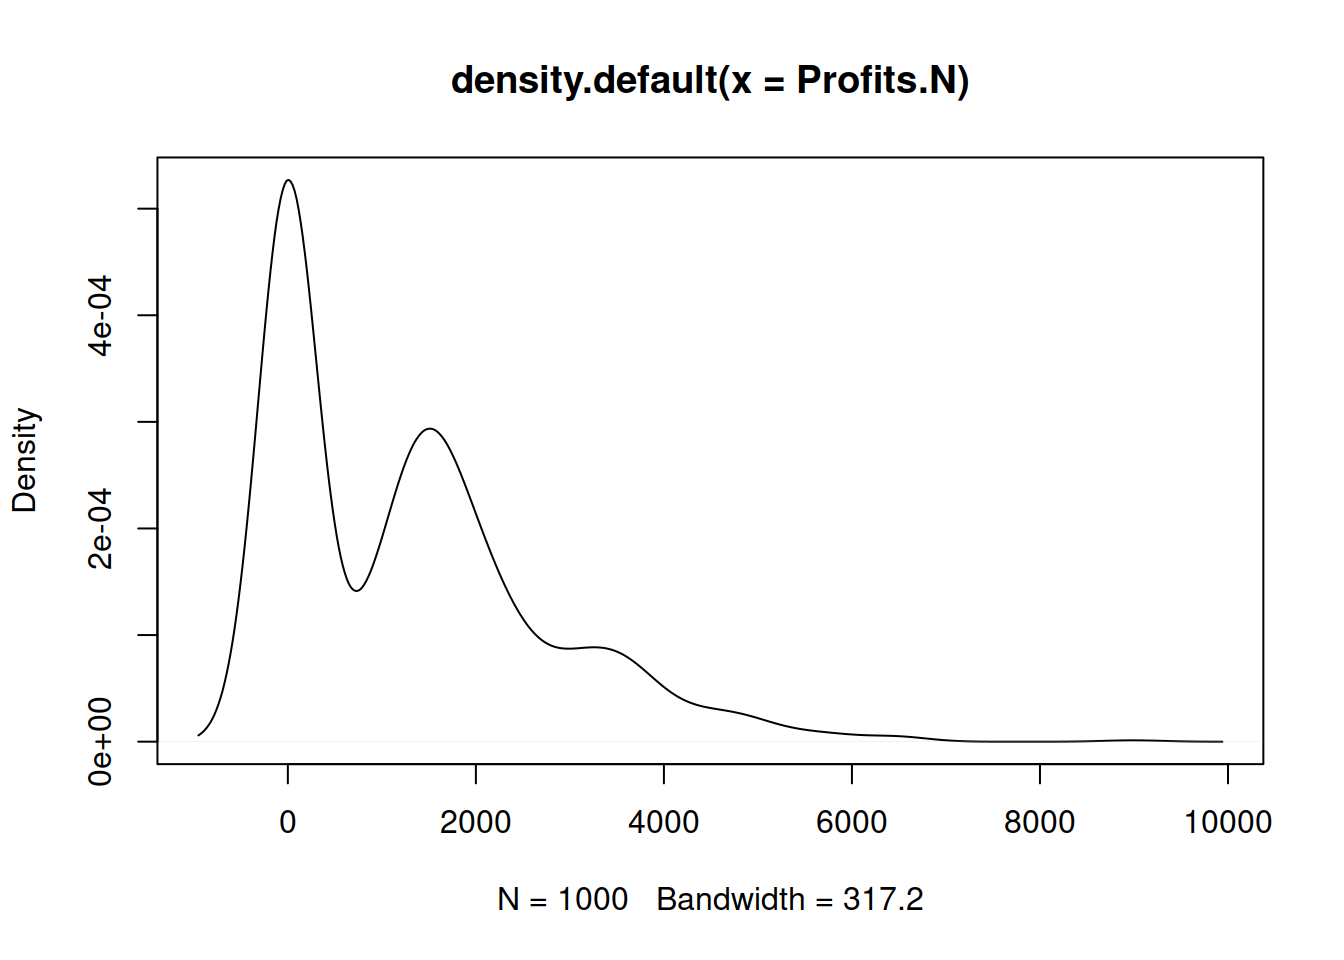
\includegraphics{Distributions_files/figure-beamer/MC1-1.pdf}

\end{frame}

\end{document}
